\documentclass[tikz,border=0pt]{standalone}
\usepackage{amsmath,amssymb}
\usetikzlibrary{arrows.meta}
\definecolor{measured}{HTML}{17365D}
\definecolor{desired}{HTML}{228833}
\begin{document}
% Schematic axis-angle correction from measured to desired orientation.
% The two outlines show the same tool face at one fixed position.
% View along the unit rotation axis u, which points towards the viewer.
% The arbitrary drawing angle has no numerical experimental meaning.
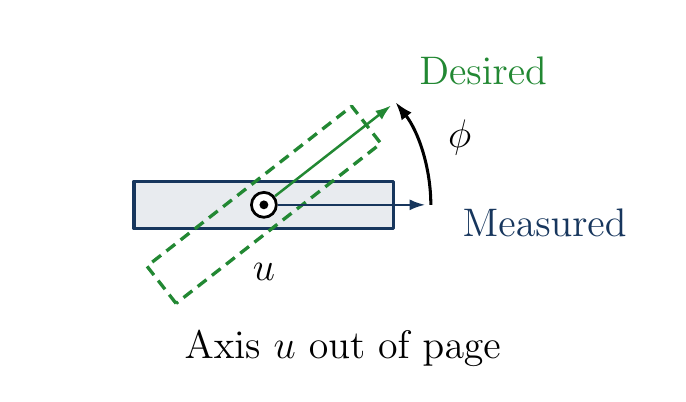
\begin{tikzpicture}[font=\fontsize{15}{18}\selectfont,
 face/.style={line width=1.2pt,line join=round},
 direction/.style={-{Latex[length=2mm,width=1.4mm]},line width=.9pt}]
\path[use as bounding box] (0,0) rectangle (8,4.4);
\coordinate (O) at (3.0,2.15);
% A filled measured face and a dashed desired outline make rotation tangible.
\begin{scope}[shift={(O)}]
  \path[face,draw=measured,fill=measured!10]
    (-1.65,-.30) rectangle (1.65,.30);
  \begin{scope}[rotate=38]
    \draw[face,desired,dash pattern=on 4pt off 2.5pt]
      (-1.65,-.30) rectangle (1.65,.30);
    \draw[direction,desired] (.18,0)--(2.05,0);
  \end{scope}
  \draw[direction,measured] (.18,0)--(2.05,0);
  % Both arc endpoints lie on the corresponding orientation directions.
  \draw[-{Latex[length=2.3mm,width=1.6mm]},line width=1.1pt,black]
    (2.12,0) arc[start angle=0,end angle=38,radius=2.12];
  \node at (19:2.63) {$\phi$};
\end{scope}
\filldraw[fill=white,draw=black,line width=1pt] (O) circle (4.5pt);
\fill[black] (O) circle (1.6pt);
\node[desired,anchor=west] at (4.85,3.85) {Desired};
\node[measured,anchor=west] at (5.4,1.92) {Measured};
\node[anchor=north] at (3.0,1.53) {$u$};
\node at (4,.33) {Axis $u$ out of page};
\end{tikzpicture}
\end{document}
